\documentclass[11pt,a4paper]{article}
\usepackage[margin=2.4cm]{geometry}
\usepackage[T1]{fontenc}
\usepackage{amsmath,amssymb}
\usepackage{booktabs}
\usepackage{siunitx}
\usepackage{pgfplots}
\pgfplotsset{compat=1.17}
\usetikzlibrary{arrows.meta,decorations.pathreplacing}
\usepackage[colorlinks=true,linkcolor=blue!50!black,urlcolor=blue!50!black]{hyperref}

\newcommand{\Ahat}{\hat{A}}
\newcommand{\Bhat}{\hat{B}}
\newcommand{\code}[1]{\texttt{#1}}
\newcommand{\incode}[1]{\par\smallskip\noindent\textit{In the code:} #1\par\smallskip}

\title{The \code{Coil} RF antenna mode in LePIC\\[4pt]
\large What it models, how every quantity is computed, and what it leaves out}
\author{LePIC modular edition}
\date{\today}

\begin{document}
\maketitle
\tableofcontents
\bigskip

%======================================================================
\section{The physical picture}
%======================================================================

An inductively coupled plasma (ICP) source with a \emph{planar} antenna
works as follows. A flat spiral coil sits just outside the chamber, behind a
dielectric window. An RF current
\begin{equation}
  I(t) = I\cos\omega t, \qquad \omega = 2\pi f_0
\end{equation}
flows in it ($f_0 = \SI{13.56}{MHz}$ here). The current produces an
oscillating magnetic field that passes through the window into the plasma.
By Faraday's law, a changing magnetic flux induces an electric field
circulating around the coil axis, $E_\theta$. Electrons are accelerated by
$E_\theta$, gain energy, and ionise the gas. This is the heating mechanism.

The plasma responds by carrying an induced current that opposes the change
of flux, like a short-circuited secondary winding of a transformer. As a
result the field cannot penetrate far: it decays over a \emph{skin depth}
$\delta$ from the window.

The \code{Coil} mode puts this picture into the PIC simulation in three
steps:
\begin{enumerate}
  \item Compute the field the \emph{actual} coil turns would produce in
        vacuum (no plasma), exactly, from magnetostatics.
  \item Multiply it by an assumed shielding factor
        $g(x) = e^{-(x-x_0)/\delta}$ to represent the plasma's screening,
        with $\delta$ recomputed from the simulated density.
  \item Apply the resulting $E_\theta$ \emph{and} RF magnetic field
        $\mathbf B_{\mathrm{RF}}$ to every particle at every push. Adjust the
        coil current $I$ every RF period so that the plasma absorbs a
        prescribed power $P_{\mathrm{abs}}$.
\end{enumerate}
The field is therefore \emph{prescribed}: it is not obtained by solving
Maxwell's equations together with the plasma current. Section~\ref{sec:limits}
discusses what this means.

\begin{figure}[ht]
\centering
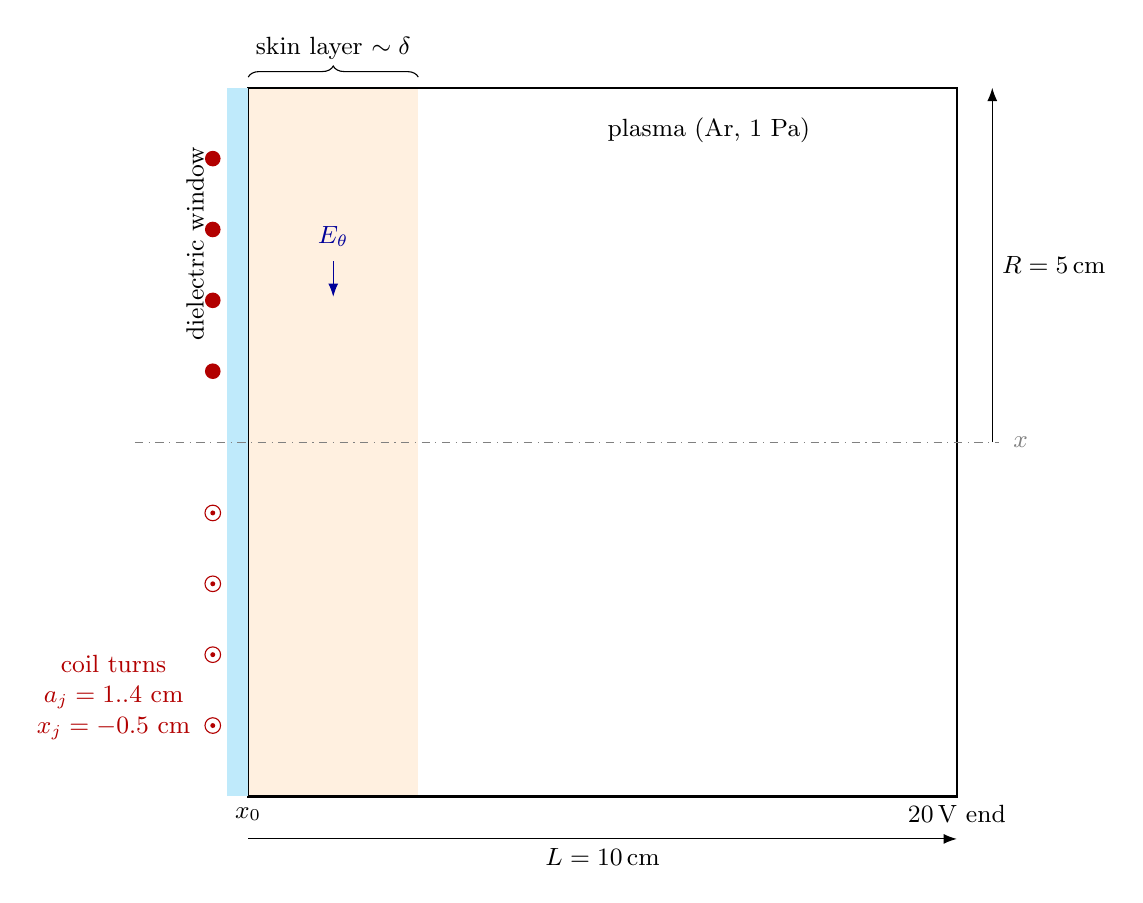
\begin{tikzpicture}[scale=0.9]
  % chamber
  \fill[orange!12] (0,-5) rectangle (2.4,5);
  \draw[thick] (0,-5) rectangle (10,5);
  \node[font=\small] at (6.5,4.4) {plasma (Ar, 1 Pa)};
  % window
  \fill[cyan!25] (-0.3,-5) rectangle (0,5);
  \node[font=\small,rotate=90] at (-0.75,2.8) {dielectric window};
  % axis
  \draw[dash dot, gray] (-1.6,0) -- (10.6,0);
  \node[font=\small,gray] at (10.9,0) {$x$};
  % turns
  \foreach \a in {1,2,3,4} {
    \fill[red!70!black] (-0.5,\a) circle (0.11);
    \draw[red!70!black, fill=white] (-0.5,-\a) circle (0.11);
    \fill[red!70!black] (-0.5,-\a) circle (0.035);
  }
  \node[font=\small,red!70!black,align=center] at (-1.9,-3.6) {coil turns\\ $a_j = 1..4$ cm\\ $x_j=-0.5$ cm};
  % labels
  \draw[-{Latex}] (0,-5.6) -- (10,-5.6) node[midway,below,font=\small] {$L = \SI{10}{cm}$};
  \draw[-{Latex}] (10.5,0) -- (10.5,5) node[midway,right,font=\small] {$R=\SI{5}{cm}$};
  \draw[decorate,decoration={brace,amplitude=4pt}] (0,5.15) -- (2.4,5.15)
       node[midway,above=3pt,font=\small] {skin layer $\sim\delta$};
  \node[font=\small] at (0,-5.25) {$x_0$};
  \node[font=\small] at (10,-5.25) {\SI{+20}{V} end};
  % E theta symbol
  \node[font=\small,blue!60!black] at (1.2,2.9) {$E_\theta$};
  \draw[blue!60!black,-{Latex}] (1.2,2.55) -- (1.2,2.05);
\end{tikzpicture}
\caption{Side view of the \code{Cyl\_coil\_RFant} case (a cut through the
axis). The four turns are circles around the $x$ axis. Each crosses the cut
twice, with the current going into the page on one side and out of it on the
other. The induced $E_\theta$ also circulates around the axis, so in this
view it points into or out of the page.}
\label{fig:geom}
\end{figure}

\paragraph{Why a magnetostatic formula is allowed.} At \SI{13.56}{MHz} the
vacuum wavelength is $c/f_0 \approx \SI{22}{m}$, about 200 times the chamber
size. Retardation (the finite speed of light) is therefore negligible. At
each instant the field is the \emph{magnetostatic} field of the
instantaneous current $I(t)$. This is the quasi-static approximation, and
the rest of this note relies on it.

%======================================================================
\section{Coordinates and coil description}
%======================================================================

The chamber axis is the $x$ axis through the centre of the $y$--$z$
cross-section. For a particle at $(x,y,z)$, define
\begin{equation}
  r = \sqrt{(y-y_{\max}/2)^2 + (z-z_{\max}/2)^2}, \qquad
  \theta = \operatorname{atan2}\!\big(z-z_{\max}/2,\; y-y_{\max}/2\big),
\end{equation}
with unit vectors
$\hat{\mathbf r} = (0,\cos\theta,\sin\theta)$ and
$\hat{\boldsymbol\theta} = (0,-\sin\theta,\cos\theta)$ in $(x,y,z)$
components. The window is the plane $x = x_0$, equal to the input
\code{xl\_pow} (clamped to $\ge 0$). The plasma is at $x > x_0$.

The real coil is a spiral. The code models it as $N$ concentric circular
loops, all coaxial with the $x$ axis. Loop $j$ has
\begin{itemize}
  \item radius $a_j$,
  \item axial position $x_j$, which must satisfy $x_j < x_0$ (behind the
        window; the code stops otherwise, because the field is singular on
        a wire),
  \item relative current $w_j$. For a series coil every turn carries the
        same current, so $w_j = 1$.
\end{itemize}

\incode{\code{input\_dir/coil.inp}: first line $N$, then one line per turn
\code{a(cm) x(cm) w}, read by \code{read\_coil\_turns} in
\code{mod\_readConditions.f90} and converted to metres. For the test case:}
\begin{verbatim}
4             ! number of turns
1.0 -0.5 1.   ! a(cm) x(cm) relative current
2.0 -0.5 1.
3.0 -0.5 1.
4.0 -0.5 1.
\end{verbatim}
The RF mode is selected in \code{conditions.inp} on the secondary-emission
line: \code{... Coil phi0 f0 phi1 f1 I R\_win}. In this mode the slot that
holds $E_0$ for the other antenna modes holds the \emph{initial guess for
the coil current $I$} (amplitude, in amperes). \code{R\_win} is used only for
the density average that sets $\delta$ (Section~\ref{sec:delta}).

%======================================================================
\section{Step 1 --- the vacuum field of the turns}
%======================================================================

\subsection{Why use the vector potential}

The geometry is axisymmetric and the coil current is purely azimuthal.
Under these conditions the vector potential has a single component,
$\mathbf A = A(r,x)\,\hat{\boldsymbol\theta}$. Everything follows from this
one scalar function:
\begin{align}
  \mathbf B &= \nabla\times\mathbf A
    &&\Rightarrow\quad
    B_r = -\frac{\partial A}{\partial x},\qquad
    B_x = \frac{1}{r}\frac{\partial (rA)}{\partial r}, \label{eq:curl}\\
  \mathbf E &= -\frac{\partial\mathbf A}{\partial t}
    &&\Rightarrow\quad E_\theta = -\frac{\partial A}{\partial t}. \label{eq:EfromA}
\end{align}
Working with $A$ has two advantages:
\begin{itemize}
  \item \textbf{$\mathbf{E}$ and $\mathbf{B}$ are automatically
        consistent.} Faraday's law
        $\nabla\times\mathbf E = -\partial_t\mathbf B$ holds identically,
        whatever $A$ is.
  \item \textbf{$\nabla\cdot\mathbf B = 0$ automatically}, because the
        divergence of a curl vanishes.
\end{itemize}
Equation \eqref{eq:EfromA} is the \emph{induced} electric field only. The
electrostatic field $-\nabla\phi$ is computed separately by LePIC's Poisson
solver, and the two are added in the particle push.

\subsection{One loop: the closed-form potential}

A circular loop of radius $a$ at $x = x_j$ carrying a current of
\SI{1}{A} has the potential (Jackson, \emph{Classical Electrodynamics},
3rd ed., eq.~5.37)
\begin{equation}
  A_{\mathrm{loop}}(r,x) = \frac{\mu_0}{\pi k}\sqrt{\frac{a}{r}}
  \left[\Big(1-\frac{k^2}{2}\Big)K(k) - E(k)\right],
  \qquad
  k^2 = \frac{4ar}{(a+r)^2 + (x-x_j)^2}.
  \label{eq:loop}
\end{equation}
\begin{itemize}
  \item $K$ and $E$ are the complete elliptic integrals of the first and
        second kind,
        $K = \int_0^{\pi/2}\! (1-k^2\sin^2\phi)^{-1/2}\,d\phi$ and
        $E = \int_0^{\pi/2}\! (1-k^2\sin^2\phi)^{1/2}\,d\phi$.
  \item $k^2\in[0,1)$ measures how close the point is to the wire. It tends
        to 1 \emph{on} the wire, where $K$ diverges logarithmically; that is
        why the turns must stay outside the plasma. It tends to 0 far away
        and on the axis.
  \item On the axis $r=0$, $A=0$ by symmetry, so $E_\theta = 0$ there. The
        induced field is always a ring.
\end{itemize}

\incode{\code{A\_loop} in \code{mod\_coilField.f90}. Two numerical details:}
\begin{itemize}
  \item \textbf{Elliptic integrals by the arithmetic--geometric mean (AGM).}
        Start with $a_0=1$, $b_0=\sqrt{1-k^2}$ and iterate
        $a_{n+1}=(a_n+b_n)/2$, $b_{n+1}=\sqrt{a_nb_n}$. Then
        $K = \pi/(2a_\infty)$, and $E$ follows from the accumulated sum
        $\sum 2^{n-1}c_n^2$ with $c_n = (a_{n-1}-b_{n-1})/2$. Convergence is
        quadratic: a few iterations reach machine precision
        (\code{ellip\_KE}).
  \item \textbf{Small-$k$ series.} When $k^2 < 10^{-3}$ (far from the wire,
        or near the axis), $(1-k^2/2)K - E$ is a difference of two nearly
        equal numbers and loses precision. The code then uses the series
        $(1-\tfrac{m}{2})K - E \simeq \tfrac{\pi}{32}m^2
        \big(1 + \tfrac34 m + \tfrac{75}{128}m^2\big)$, with $m=k^2$.
\end{itemize}

\subsection{All turns: superposition and the table}

Magnetostatics is linear, so the coil's potential is the sum over turns.
Normalising by the current gives a fixed shape function, \emph{per ampere}:
\begin{equation}
  \Ahat(r,x) = \sum_{j=1}^{N} w_j\,A_{\mathrm{loop}}(r,x;\,a_j,x_j)
  \qquad[\si{T.m/A}].
\end{equation}
The actual potential is $A = I(t)\,\Ahat$. Because $\Ahat$ does not depend
on time or on the plasma, it is computed \textbf{once at start-up} on a 2D
grid in $(r,x)$ and stored as a table:
\begin{itemize}
  \item spacing $\Delta r = \tfrac12\min(h_y,h_z)$ and
        $\Delta x = \tfrac12 h_x$, half the PIC cell. For the test case
        that is \SI{0.65}{mm} and \SI{0.625}{mm};
  \item $r$ from 0 to the corner of the $y$--$z$ box, and $x$ over the
        whole domain, so every particle position is covered.
\end{itemize}

\subsection{The magnetic field: the flux function $\psi = r\Ahat$}
\label{sec:psi}

$\Bhat$ could be computed analytically from more elliptic-integral
formulas. The code instead differentiates the tabulated potential through
the \emph{flux function}
\begin{equation}
  \psi(r,x) = r\,\Ahat(r,x),
\end{equation}
which is the magnetic flux through a circle of radius $r$, divided by
$2\pi$. From \eqref{eq:curl}:
\begin{equation}
  \Bhat_r = -\frac{1}{r}\frac{\partial\psi}{\partial x},\qquad
  \Bhat_x =  \frac{1}{r}\frac{\partial\psi}{\partial r}.
  \label{eq:Bpsi}
\end{equation}
Both derivatives are taken by second-order central differences on the
table. This gives the divergence-free property exactly on the discrete
grid. Written with the same central operators,
\begin{equation}
  \nabla\cdot\Bhat = \frac{1}{r}\frac{\partial(r\Bhat_r)}{\partial r}
                   + \frac{\partial\Bhat_x}{\partial x}
  = -\frac{1}{r}\,\partial_r\partial_x\psi + \frac{1}{r}\,\partial_x\partial_r\psi = 0,
\end{equation}
because central differences in $r$ and in $x$ commute. The result is zero
to round-off, not merely to $O(\Delta^2)$.

\paragraph{On the axis.} $\Bhat_x = \psi_r/r$ is $0/0$ at $r=0$. Near the
axis the flux through a small circle is $\psi \simeq \tfrac12\Bhat_x(0,x)\,r^2$,
so $\Bhat_x(0,x) = \lim_{r\to0}2\psi/r^2$. The code evaluates this at the
first node, $2\psi(\Delta r)/\Delta r^2$. $\Ahat$ and $\Bhat_r$ are set to
0 on the axis.

\incode{\code{CoilField\%build}: $\psi$ is filled with one extra node on
every side so that all table nodes use central differences, and the loop
over $x$ is OpenMP-parallel. The arrays \code{Ahat}, \code{Brhat} and
\code{Bxhat} have shape \code{(0:nr, 0:nx)}.}

\subsection{Start-up checks}

At start-up \code{CoilField\%self\_check} prints three independent tests of
the table:
\begin{enumerate}
  \item \textbf{On-axis field against the exact formula.} On the axis the
        field of a loop is elementary,
        $B_x = \mu_0 a^2 / \big(2(a^2+(x-x_j)^2)^{3/2}\big)$. The tabulated
        $\Bhat_x(0,x)$ is compared with the sum of these. The relative
        error is about $10^{-3}$: second order in $\Delta r$, from the axis
        limit above.
  \item \textbf{Far field against a dipole.} At distance $R = 100a$ a loop
        looks like a magnetic dipole of moment $\pi a^2$, with
        $A \to \mu_0 a^2\sin\vartheta/(4R^2)$. The loop formula agrees to
        about $10^{-4}$. This checks \eqref{eq:loop} and the AGM.
  \item \textbf{Discrete $\nabla\cdot\Bhat$}, normalised as
        $\max|\nabla\cdot\Bhat|\,\Delta/\max|\Bhat|$. The result is about
        $10^{-17}$, as argued in Section~\ref{sec:psi}.
\end{enumerate}
The vacuum table is written to \code{Output/coil\_field.dat}, one line per
node: $r$ (cm), $x$ (cm), $\Ahat$, $\Bhat_r$, $\Bhat_x$, all per ampere and
without shielding. It can be plotted directly, e.g.\ with gnuplot
\code{splot} using columns 1:2:3.

\subsection{What the vacuum field looks like here}

Figure~\ref{fig:vac} shows the field of the four test-case turns,
normalised.
\begin{itemize}
  \item \textbf{Radially}, $E_\theta$ at the window rises from 0 on the
        axis, peaks at $r\approx\SI{3}{cm}$ and is down to 54\% at the wall.
  \item \textbf{Axially}, even without any plasma, the field of a coil of
        this size falls to $1/e$ at \SI{1.9}{cm} from the window: moving
        away from a set of loops, their contributions weaken quickly.
  \item \textbf{Magnitudes per ampere (vacuum, at the window):}
        $\max\,\omega\Ahat \approx \SI{73}{V/m}$ and
        $\Bhat_x(0,x_0) \approx \SI{1.1e-4}{T}$ (\SI{1.1}{G}).
\end{itemize}

\begin{figure}[ht]
\centering
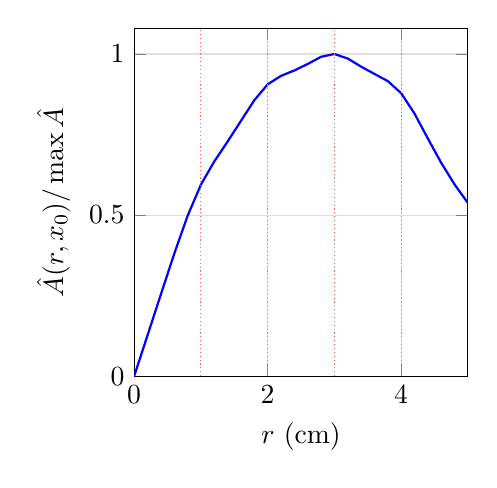
\begin{tikzpicture}
\begin{axis}[
  width=0.48\textwidth, height=6cm,
  xlabel={$r$ (cm)}, ylabel={$\Ahat(r,x_0)/\max\Ahat$},
  xmin=0, xmax=5, ymin=0, ymax=1.08,
  grid=major, grid style={gray!25}]
\addplot[thick, blue] coordinates {
(0.0,0.0000)(0.2,0.1267)(0.4,0.2537)(0.6,0.3796)(0.8,0.4974)(1.0,0.5944)
(1.2,0.6664)(1.4,0.7282)(1.6,0.7924)(1.8,0.8565)(2.0,0.9058)(2.2,0.9322)
(2.4,0.9488)(2.6,0.9691)(2.8,0.9913)(3.0,1.0000)(3.2,0.9858)(3.4,0.9607)
(3.6,0.9381)(3.8,0.9159)(4.0,0.8783)(4.2,0.8150)(4.4,0.7376)(4.6,0.6621)
(4.8,0.5951)(5.0,0.5373)};
\foreach \a in {1,2,3,4} { \edef\tmp{\noexpand\draw[red!60, densely dotted] (axis cs:\a,0) -- (axis cs:\a,1.08);} \tmp }
\end{axis}
\end{tikzpicture}
\hfill
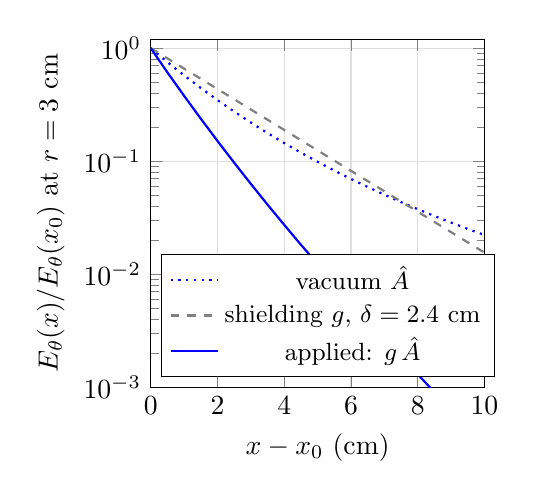
\begin{tikzpicture}
\begin{axis}[
  width=0.48\textwidth, height=6cm,
  xlabel={$x - x_0$ (cm)}, ylabel={$E_\theta(x)/E_\theta(x_0)$ at $r=3$ cm},
  xmin=0, xmax=10, ymode=log, ymin=1e-3, ymax=1.2,
  legend pos=south west, legend style={font=\small},
  grid=major, grid style={gray!25}]
\addplot[thick, blue, dotted] coordinates {
(0.0,1.0000)(0.5,0.7512)(1.0,0.5743)(1.5,0.4441)(2.0,0.3473)(2.5,0.2747)
(3.0,0.2195)(3.5,0.1773)(4.0,0.1445)(4.5,0.1189)(5.0,0.0987)(5.5,0.0825)
(6.0,0.0696)(6.5,0.0591)(7.0,0.0505)(7.5,0.0434)(8.0,0.0376)(8.5,0.0327)
(9.0,0.0286)(9.5,0.0251)(10.0,0.0222)};
\addlegendentry{vacuum $\Ahat$}
\addplot[thick, gray, dashed, domain=0:10, samples=41] {exp(-x/2.4)};
\addlegendentry{shielding $g$, $\delta=2.4$ cm}
\addplot[thick, blue] coordinates {
(0.0,1.0000)(0.5,0.6099)(1.0,0.3786)(1.5,0.2377)(2.0,0.1509)(2.5,0.0969)
(3.0,0.0629)(3.5,0.0412)(4.0,0.0273)(4.5,0.0182)(5.0,0.0123)(5.5,0.0083)
(6.0,0.0057)(6.5,0.0039)(7.0,0.0027)(7.5,0.0019)(8.0,0.0013)(8.5,0.0009)
(9.0,0.0007)(9.5,0.0005)(10.0,0.0003)};
\addlegendentry{applied: $g\,\Ahat$}
\end{axis}
\end{tikzpicture}
\caption{Field shape of the test-case coil. Left: radial profile at the
window; dotted red lines mark the turn radii. Right: decay away from the
window at the radius of the peak, separated into the vacuum geometry, the
plasma shielding, and their product (what the particles see).}
\label{fig:vac}
\end{figure}

%======================================================================
\section{Step 2 --- plasma shielding}
%======================================================================

\subsection{The shielding factor}

Inside the plasma the induced current screens the field. The code does not
compute this current. It assumes the screening multiplies the vacuum
potential by an exponential in the distance from the window:
\begin{equation}
  A(r,x) = g(x)\,\Ahat(r,x),\qquad
  g(x) = \begin{cases} e^{-(x-x_0)/\delta}, & x > x_0,\\ 1, & x\le x_0.\end{cases}
\end{equation}

\subsection{The magnetic field is re-derived from the shielded potential}

$\mathbf B$ is \emph{not} computed as $g\,\Bhat$. That would no longer be
the curl of anything and would break $\nabla\cdot\mathbf B = 0$ and
Faraday's law. Instead, \eqref{eq:curl} is applied to $g\Ahat$, using
$g' = -g/\delta$:
\begin{align}
  B_r &= -\frac{\partial (g\Ahat)}{\partial x}
       = -g\frac{\partial\Ahat}{\partial x} - g'\Ahat
       = g\left(\Bhat_r + \frac{\Ahat}{\delta}\right), \\
  B_x &= \frac{1}{r}\frac{\partial (r g\Ahat)}{\partial r} = g\,\Bhat_x .
\end{align}
The extra term $g\Ahat/\delta$ in $B_r$ is real physics within the model. A
field that falls off quickly along $x$ must have field lines bending
outward, which is a radial component. For the test case at $r=\SI{3}{cm}$
it is $\Ahat/\delta \approx \SI{3.6e-5}{T/A}$ (\SI{0.36}{G/A}).

\incode{\code{CoilField\%eval(xp, rp, x0, delta, A, Br, Bx)}: bilinear
interpolation of the three tables at $(r,x)$, then the shielding above.
$g$ is applied at evaluation time, so the table never has to be rebuilt
when $\delta$ changes.}

\subsection{How $\delta$ is chosen}
\label{sec:delta}

Every RF period, $\delta$ is set to the \emph{collisionless skin depth}
\begin{equation}
  \delta = \frac{c}{\omega_{pe}},\qquad
  \omega_{pe} = \sqrt{\frac{\langle n_e\rangle e^2}{\varepsilon_0 m_e}},
  \qquad
  \delta \approx \SI{5.3}{cm}\times\sqrt{\frac{\SI{1e16}{m^{-3}}}{\langle n_e\rangle}},
\end{equation}
where $\langle n_e\rangle$ is the mean electron density over all grid nodes
with $r\le R_{\mathrm{win}}$ inside the heating slab. The true
$\varepsilon_0$ is used even when the run rescales it with $k_{\varepsilon_0}$.
At $5\times10^{16}$\,m$^{-3}$ this gives $\delta\approx\SI{2.4}{cm}$.

\paragraph{When is this formula appropriate?} The collisionless formula
assumes the electron--neutral collision frequency $\nu_m$ is below
$\omega$. At \SI{1}{Pa} in argon with $T_e\approx\SI{3}{eV}$,
$\nu_m \sim n_g\sigma v \sim \SI{2e7}{s^{-1}}$, against
$\omega = \SI{8.5e7}{s^{-1}}$: marginally satisfied. Electrons also travel
$v_{th}/\omega\approx\SI{1}{cm}$ per radian of RF phase, comparable to
$\delta$. The real screening is therefore partly \emph{non-local}
(the anomalous skin effect), which a single exponential cannot represent.
This is one of the model's main approximations.

\incode{\code{update\_rf\_convergence} in \code{mod\_state.f90}. The value
is stored in \code{State\%gams}, printed as ``skin depth gam(cm)'', and
logged to \code{Output/skin\_depth.dat}.}

%======================================================================
\section{Step 3 --- the fields seen by the particles}
%======================================================================

\subsection{Putting in the time dependence}

With $A(t) = I\cos\omega t\;g\Ahat$, \eqref{eq:EfromA} and \eqref{eq:curl}
give
\begin{equation}
  \boxed{\;
  E_\theta = \omega I\,g\Ahat\,\sin\omega t, \qquad
  \mathbf B_{\mathrm{RF}} = I\big(B_r\hat{\mathbf r} + B_x\hat{\mathbf x}\big)\cos\omega t
  \;}
  \label{eq:fields}
\end{equation}
\begin{itemize}
  \item $E_\theta$ is proportional to $\omega$, because it is induced by the
        \emph{rate of change} of the flux. At fixed current, a higher
        frequency gives a stronger electric field.
  \item $\mathbf E$ and $\mathbf B$ are \SI{90}{\degree} out of phase. $E$
        is largest when the current, and hence $B$, passes through zero.
  \item In Cartesian components,
        $E_y = -E_\theta\sin\theta$ and $E_z = E_\theta\cos\theta$;
        $B_y = B_r\cos\theta$, $B_z = B_r\sin\theta$, and $B_x$ is along the axis.
\end{itemize}

\incode{\code{compute\_coil\_field} in \code{mod\_particleMover.f90}. It is
called only for particles in cells between \code{ixl\_pow} and
\code{ixr\_pow} (the ``RF region''; here the whole chamber).}

\subsection{The push: why Boris is used}

The particles are advanced by the leapfrog scheme. The total electric field
is the electrostatic field gathered from the grid plus the RF field,
$\mathbf E = -\nabla\phi + E_\theta\hat{\boldsymbol\theta}$. The magnetic
field is $\mathbf B = \mathbf B_0 + \mathbf B_{\mathrm{RF}}$, where
$\mathbf B_0$ is any static map; it is zero in the test case. A magnetic
force $q\mathbf v\times\mathbf B$ needs a rotation step, so in \code{Coil}
mode \emph{every species} goes through the \textbf{Boris} push:
\begin{enumerate}
  \item half electric kick:
        $\mathbf v^- = \mathbf v^{n-1/2} + \frac{q\Delta t}{2m}\mathbf E$;
  \item rotation about $\mathbf B$:
        $\mathbf t = \frac{q\Delta t}{2m}\mathbf B$,
        $\mathbf v' = \mathbf v^- + \mathbf v^-\times\mathbf t$,
        $\mathbf v^+ = \mathbf v^- + \mathbf v'\times\frac{2\mathbf t}{1+t^2}$;
  \item second half kick:
        $\mathbf v^{n+1/2} = \mathbf v^+ + \frac{q\Delta t}{2m}\mathbf E$;
  \item position:
        $\mathbf x^{n+1} = \mathbf x^n + \Delta t\,\mathbf v^{n+1/2}$.
\end{enumerate}
The rotation preserves $|\mathbf v|$ exactly, so the magnetic field does no
work, as in the physics. The electrostatic field is still gathered with
the energy-conserving (EC-PIC) scheme when \code{push = energy}. The Boris
step changes only how the magnetic force is applied.

\paragraph{Is $\mathbf B_{\mathrm{RF}}$ important?} Compare the electron
cyclotron frequency in it, $f_{ce} = eB/(2\pi m_e) \approx
\SI{2.8}{MHz}$ per gauss, with $f_0$. For a current of a few amperes,
$B_{\mathrm{RF}}$ near the window is a few gauss, so
$f_{ce}\sim$ 5--12\,MHz, comparable to \SI{13.56}{MHz}. Electrons near the
window are therefore noticeably deflected during each RF cycle. This
$\mathbf v\times\mathbf B$ force (and the ponderomotive and second-harmonic
effects it produces) is the main physics that \code{Coil} has and a pure
$E_\theta$ model lacks.

\incode{\code{move\_and\_bc\_boris}; $\mathbf B_{\mathrm{RF}}$ is added to
the static field just before the rotation, and the rotation is switched on
even where $\mathbf B_0$ is negligible.}

%======================================================================
\section{Step 4 --- absorbed power and the current controller}
%======================================================================

\subsection{Measuring the absorbed power}

The power the RF field gives to the plasma is the work done by
$E_\theta$. The magnetic force does no work, so $\mathbf B_{\mathrm{RF}}$
does not enter. At every push, for every particle in the RF region,
\begin{equation}
  \Delta W = N_m\, q\, E_\theta\, \bar v_\theta\,\Delta t,
  \qquad
  \bar v_\theta = \tfrac12\big(v_\theta^{n-1/2} + v_\theta^{n+1/2}\big),
\end{equation}
where $N_m$ is the macroparticle weight. The time-centred velocity makes
$\Delta W$ consistent with the leapfrog energy change. Summed over particles
(and MPI ranks) and divided by the RF period, this gives
$P_{\mathrm{RF}}$, the ``\code{<P\_RF>(W)}'' in the log and the
\code{Pabs} column of \code{Ptot.dat}.

\subsection{Controlling the current}

The user prescribes the absorbed power, $P_{\mathrm{abs}}$ (first value on
the \code{Pabs} line of \code{conditions.inp}), not the current. At the end
of each RF period, every $n_{\mathrm{RF}} = 1/(f_0\Delta t)$ steps
($\approx 4850$ here), the current is rescaled:
\begin{equation}
  I \;\leftarrow\; I\,\sqrt{\frac{P_{\mathrm{abs}}}{P_{\mathrm{RF}}}} .
\end{equation}
The reasoning: at a fixed plasma state $E\propto I$ and the absorbed power
is $\propto E^2$, so $P\propto I^2$, and the square root makes one step
exact if the plasma did not change. In practice the plasma does respond, so
a few periods are needed. In the 40$^3$ smoke test the current went from
\SI{10}{A} to \SI{1.86}{A} and the power settled at \SI{15.1}{W} against a
target of \SI{15}{W} within six periods. The controller has no damping or
limit (the same law as the legacy code), so a run where the plasma is
collapsing can drive $I$ upwards without bound. Watch \code{I\_coil(A)} in
the log.

$I$ is a \textbf{peak} current per turn (amplitude, not rms). For a real
antenna, compare $I/\sqrt2$ with rms meter readings.

\incode{The current is stored in \code{cfg\%E0\_RF}, the same variable
that holds $E_0$ in the other modes, and the log prints
``\code{it=..., I\_coil(A)=..., <P\_RF>(W)=..., <np>(/m\^{}3)=..., skin depth
gam(cm)=...}'' once per period. Both $\delta$ and $I$ are updated in the
same call, \code{update\_rf\_convergence}.}

%======================================================================
\section{What the model does \emph{not} include}
\label{sec:limits}
%======================================================================

\begin{enumerate}
  \item \textbf{No self-consistent field.} The plasma current is never fed
        back into Maxwell's equations. The shielding is the assumed
        exponential $g(x)$, with the same $\delta$ at all radii and the
        collisionless formula, whatever the actual density profile. The
        true field obeys
        $\nabla^2\mathbf A - i\omega\mu_0\sigma\mathbf A = -\mu_0\mathbf J_{\mathrm{coil}}$
        with the plasma conductivity $\sigma$; that is the planned
        ``Phase~2''.
  \item \textbf{Strictly, the model fields satisfy Faraday's law but not
        Ampère's law in the plasma.} $\nabla\times\mathbf B_{\mathrm{RF}}$
        implies a current density $\mathbf J = \nabla\times\mathbf B/\mu_0$
        that is not the current the particles carry. The fields are
        geometrically consistent, not dynamically.
  \item \textbf{No capacitive coupling.} A real coil also has an RF voltage
        along it, which couples electrostatically through the window
        (the E-mode). Only the inductive (H-mode) field is modelled.
  \item \textbf{Concentric loops instead of a spiral.} The small radial
        pitch of a real spiral and the leads are ignored. All turns carry
        the same current in phase.
  \item \textbf{Circuit not modelled.} The coil voltage, impedance and
        matching network are not computed; only the current needed for the
        target power is.
  \item \textbf{Momentum diagnostic.} The RF impulse recorded for the
        momentum balance (\code{Fabs}) contains $qE_{\mathrm{RF}}\Delta t$
        but not the $q\mathbf v\times\mathbf B_{\mathrm{RF}}\Delta t$ part.
        The power diagnostic is complete, because $\mathbf B$ does no work.
\end{enumerate}

%======================================================================
\section{Summary: from input to particle push}
%======================================================================

\begin{center}
\renewcommand{\arraystretch}{1.3}
\begin{tabular}{@{}p{0.22\textwidth}p{0.44\textwidth}p{0.27\textwidth}@{}}
\toprule
When & What & Where \\
\midrule
Input & turns $(a_j,x_j,w_j)$; RF mode \code{Coil}; initial $I$;
        $P_{\mathrm{abs}}$; $R_{\mathrm{win}}$
      & \code{coil.inp}, \code{conditions.inp} \\
Start-up & tabulate $\Ahat$ from \eqref{eq:loop}; $\Bhat$ from $\psi=r\Ahat$;
           checks; write table
         & \code{mod\_coilField.f90} \\
Every push & interpolate table; apply $g(x)$; form $E_\theta$,
             $\mathbf B_{\mathrm{RF}}$ \eqref{eq:fields}; Boris push;
             accumulate $qE_\theta\bar v_\theta$
           & \code{mod\_particleMover.f90} \\
Every RF period & $\langle n_e\rangle\to\delta=c/\omega_{pe}$;
                  $I\leftarrow I\sqrt{P_{\mathrm{abs}}/P_{\mathrm{RF}}}$; log
                & \code{update\_rf\_convergence} \\
\bottomrule
\end{tabular}
\end{center}

\paragraph{Symbols and code names.}
\begin{center}
\begin{tabular}{@{}lll@{}}
\toprule
Symbol & Meaning & Code \\
\midrule
$I$ & coil current amplitude (A) & \code{cfg\%E0\_RF} \\
$\omega$ & $2\pi f_0$ & \code{omega\_RF} \\
$x_0$ & window position & \code{xl\_pow} $\to$ \code{x0} \\
$\delta$ & skin depth & \code{State\%gams} \\
$\Ahat,\ \Bhat_r,\ \Bhat_x$ & vacuum tables per ampere & \code{coil\%Ahat}, \code{Brhat}, \code{Bxhat} \\
$a_j, x_j, w_j$ & turn radius, position, weight & \code{cfg\%coil\_a}, \code{coil\_x}, \code{coil\_w} \\
$R_{\mathrm{win}}$ & radius of the $\langle n_e\rangle$ disk & \code{cfg\%R\_win} $\to$ \code{R\_ahp} \\
$P_{\mathrm{abs}}$ & target absorbed power & \code{cfg\%Pabs} \\
$P_{\mathrm{RF}}$ & measured absorbed power & \code{State\%P\_RF} (summed) \\
\bottomrule
\end{tabular}
\end{center}

\end{document}
